\section{Workflow}\label{sec:Workflow}

\noindent A user or resource manager needs to follow two steps in order to visualize and modify \acrshort*{RDF} resources within the prototype. First, they need to create or edit a board configuration along with the desired board and card component resources within eccenca’s \textit{DataManager}. Then, they can select the board in the prototype, and start to explore or edit resources. Editing resources can either be performed by relocating cards on the board (which would update the resources column property), or by clicking on a card (which would open eccenca’s \tns{SHACLINE} modal window). Since the board configuration was already introduced within \autoref{sec:BoardConfiguration} (specification), including its visual representation (\autoref{fig:BoardConfigs}), the following section will showcase the final stage of the prototype, as illustrated by a series of screenshots showing different \acrshort*{UI} components and use cases.

To begin with, \autoref{fig:01InitialBoardState} shows the initial application state, waiting for the user to select a board configuration (i.e., one of the four use cases in the select box). This state corresponds to the process flow of \autoref{fig:RMBProcessFlow} after fetching all board configurations ({\small \hyperref[ssec:QS-A]{\(\mathcal{A}\)}}).



\begin{figure}[H]
\centering
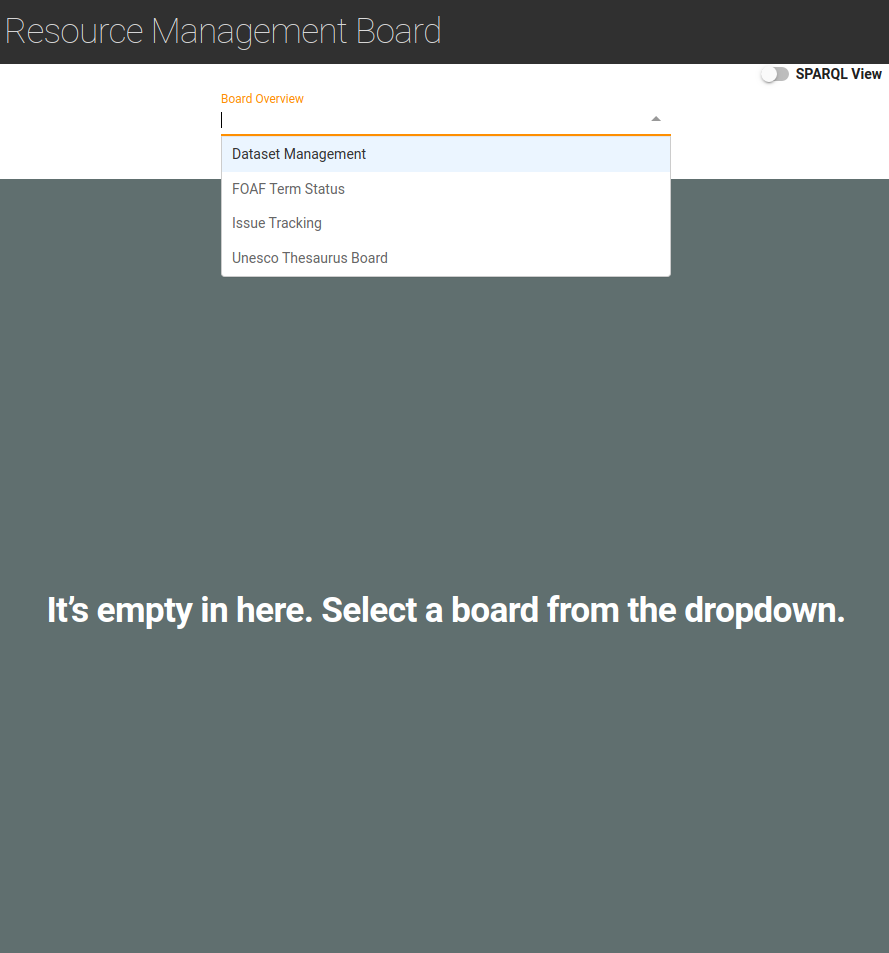
\includegraphics[width=0.7\textwidth]{img/01-InitialBoard.png}
	\caption[\tns{RMB} — Initial Board State]{Initial board state of the \tns{RMB}. }
	\label{fig:01InitialBoardState}
\end{figure}

\newpage

\noindent \autoref{fig:02SPARQLView} shows the \tns{SPARQL} View component, which expands above the board selection box. To reveal this information, the user needs to toggle the \tns{SPARQL} View at the top right corner. In this instance, the component contains the auto-composed query to request the data for the first use case (\tns{FOAF} Terms Status). The query corresponds to stage {\small \hyperref[ssec:QS-C]{\(\mathcal{C}\)}} of \autoref{fig:RMBProcessFlow} and likewise to \autoref{lst:SPARQLGetBoardsDataDemo}.

\begin{figure}[H]
\centering
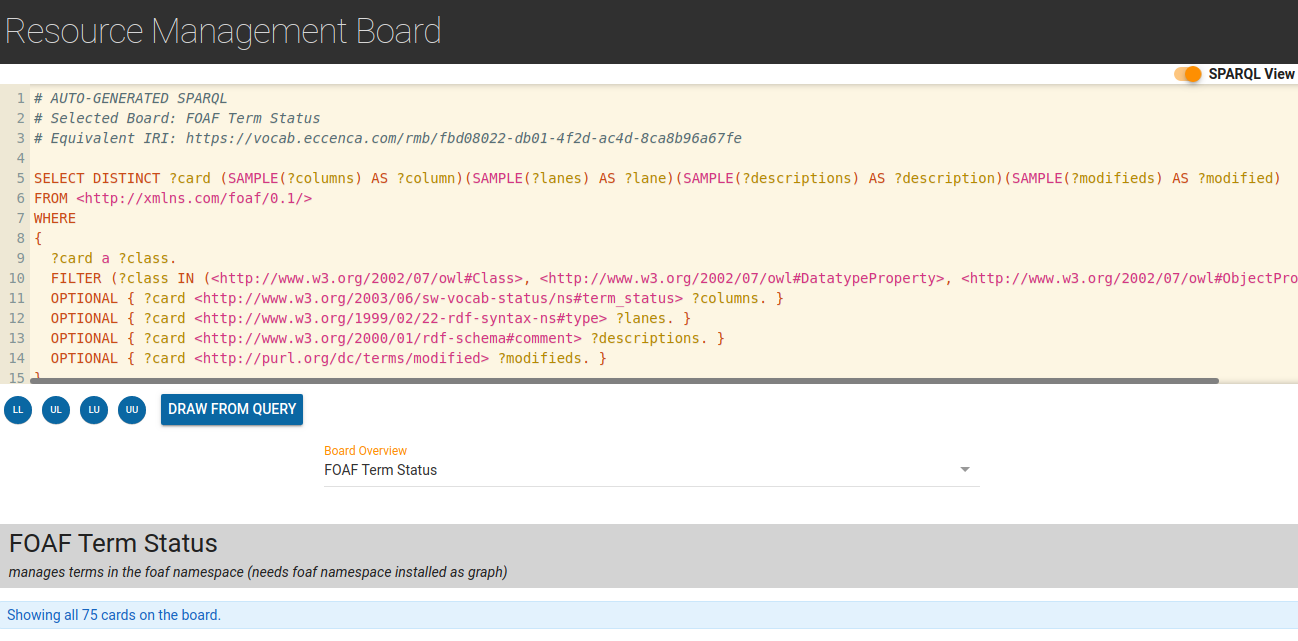
\includegraphics[width=0.99\textwidth]{img/02-SPARQL-View.png}
	\caption[\tns{RMB} — \tns{SPARQL} View]{\tns{SPARQL} View component with the auto composed query for the first use case.}
	\label{fig:02SPARQLView}
\end{figure}


\noindent \autoref{fig:03FOAF} shows the board for the first use case (\tns{FOAF} Term Status). Since there was no explicit limit set, the implicit limit (100) is above the number of resources being depicted as cards. Therefore, the infobox provides the corresponding information.

\begin{figure}[H]
\centering
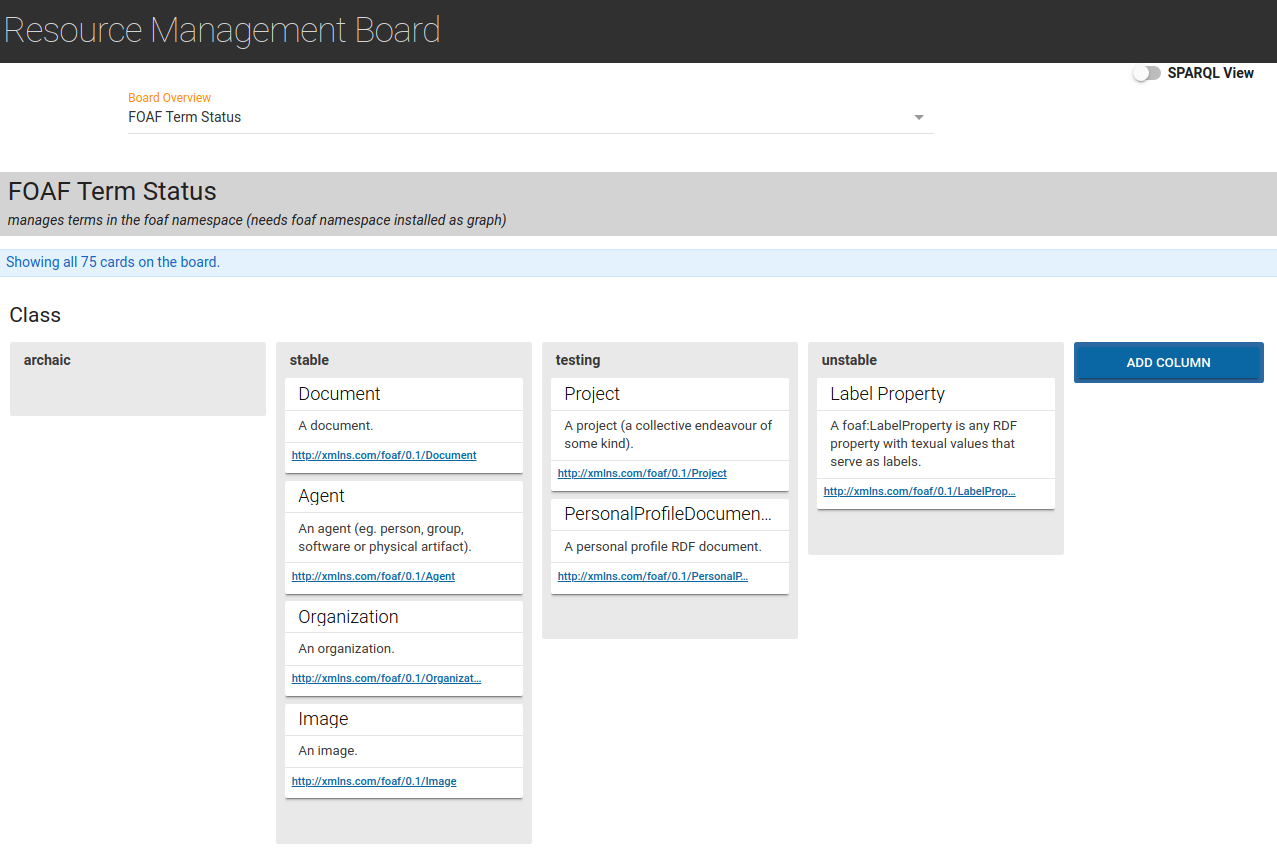
\includegraphics[width=0.99\textwidth]{img/03-FOAF.png}
	\caption[\tns{RMB} of Use Case 1]{\tns{RMB} of use case 1. Only the first swimlane is depicted.}
	\label{fig:03FOAF}
\end{figure}

\newpage

\noindent \autoref{fig:04UNESKOS} shows the board for the second use case. Since the terms from the \tns{UNESKOS} graph do not contain the defined column property \acrshort{vs}\texttt{term\_status}, the cards are allocated in the fallback column \textit{no property}. As outlined in this use case (see \autoref{ssec:UseCase2-Unesco Thesaurus}), users may then start to create term statuses from scratch and assign cards correspondingly (as depicted).

Since there was no explicit limit defined, the implicit limit avoids loading over 4.000 cards on the board. However, if a user wants to increase the limit, they can either set a higher explicit limit in the board configuration or use the \tns{SPARQL} View to increase the \texttt{LIMIT} and redraw the board.


\begin{figure}[H]
\centering
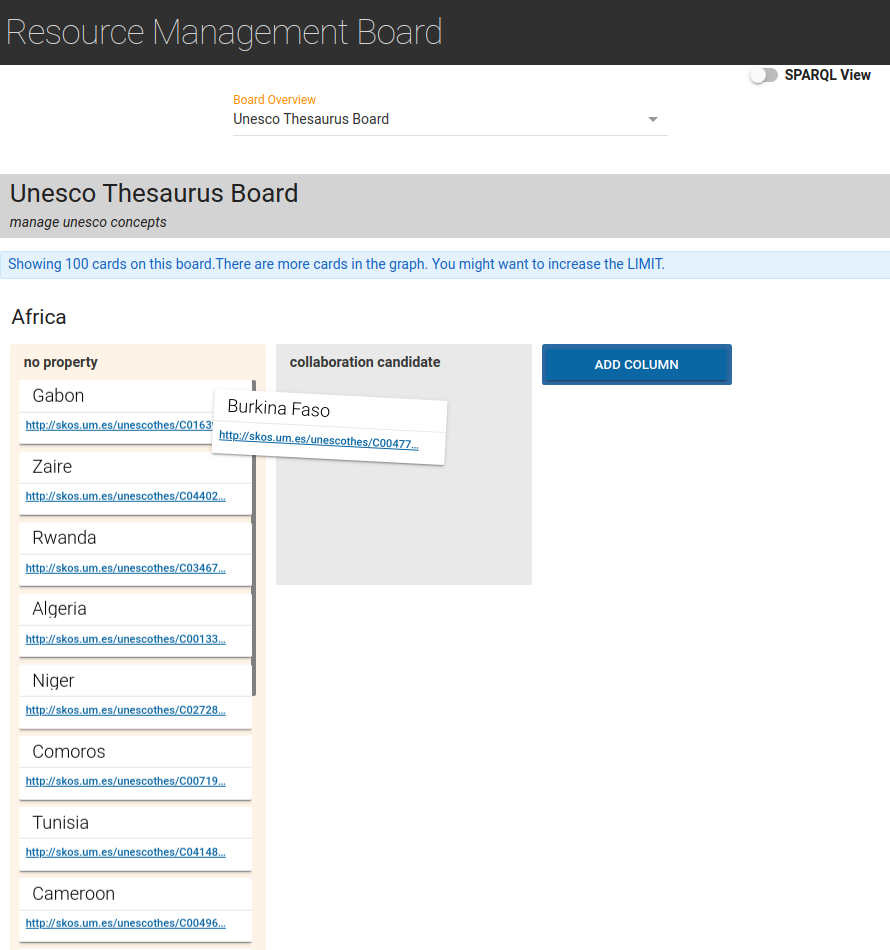
\includegraphics[width=0.80\textwidth]{img/04-UNESKOS.png}
	\caption[\tns{RMB} of Use Case 2]{\tns{RMB} of use case 2.}
	\label{fig:04UNESKOS}
\end{figure}


\newpage

\noindent \autoref{fig:04UNESKOS} shows the board for the third use case. This use case focused on the use of additional properties, as outlined  \autoref{ssec:UseCase3-DatasetMGMT}. Additional properties allow to display an arbitrary amount of properties defined in the card’s resource. Additional properties are displayed as key-value pairs, as specified in \autoref{fig:CardTemplateMDL} (A\libertineLF3\libertineOsF).

The card \textit{RND Spending} was moved from the column \textit{published} to the column \textit{needs approval}, which was triggering the real-time events to recolor the card and set the modified timestamp to \textit{just now}, as requested in \tns{FR}\textsubscript{26/27}. Both events are only temporarily, meaning that after refreshing the board, the card will have its default background color and a relative timestamp (e.g., \textit{Modified: a minute ago}).



\begin{figure}[H]
\centering
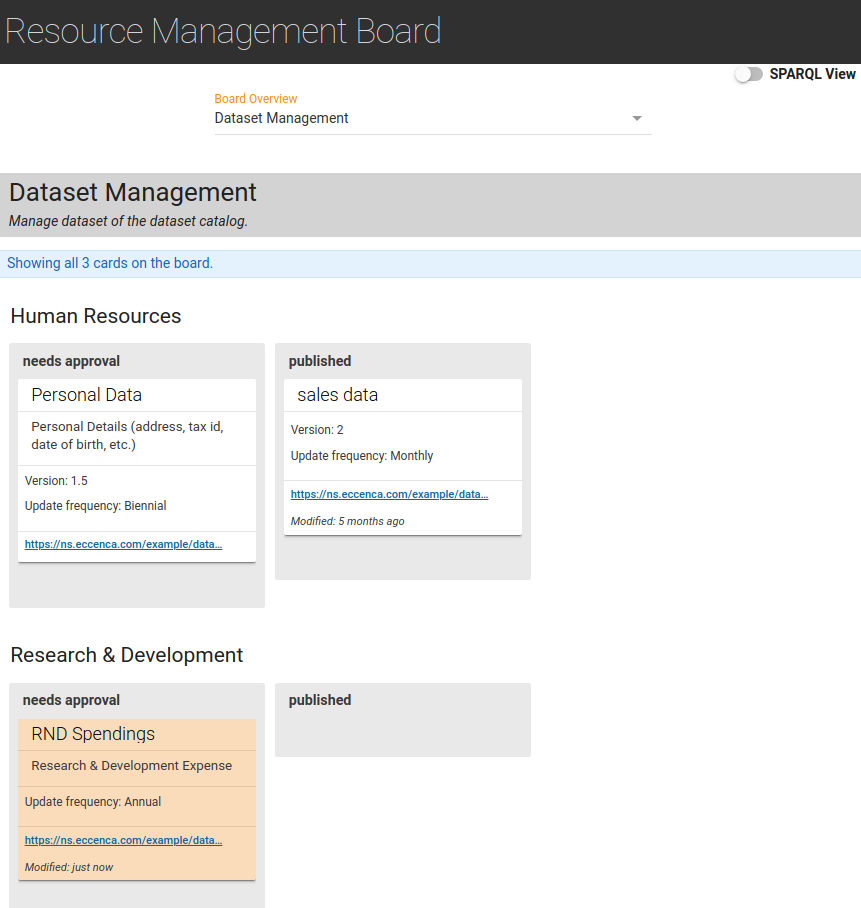
\includegraphics[width=0.85\textwidth]{img/05-DatasetMGMT.png}
	\caption[\tns{RMB} of Use Case 3]{\tns{RMB} of use case 3, demonstrating additional properties and real-time events.}
	\label{fig:05DatasetMGMT}
\end{figure}

\newpage


\noindent \autoref{fig:04UNESKOS} shows the board for the last use case, using a subset of the \tns{DOAP} vocabulary to specify columns and lanes, as outlined in \autoref{ssec:UseCase4IssueTracking}.


\begin{figure}[H]
\centering
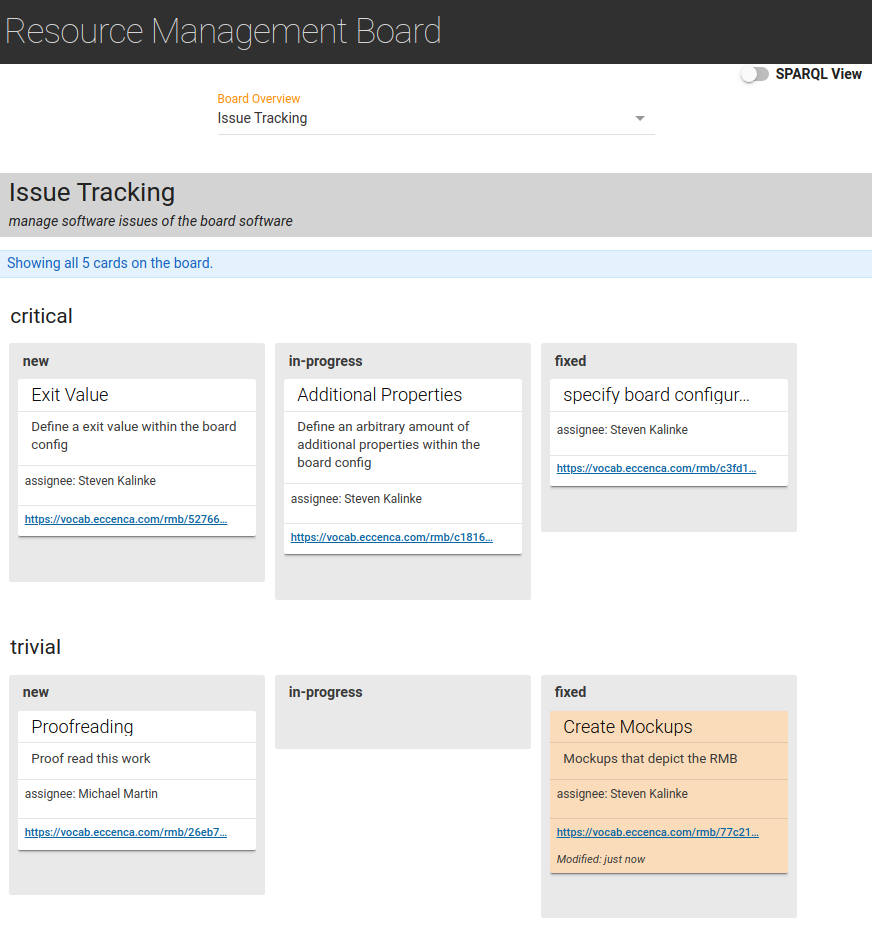
\includegraphics[width=0.90\textwidth]{img/06-IssueTracking.png}
	\caption[\tns{RMB} of Use Case 4]{\tns{RMB} of use case 4.}
	\label{fig:06IssueTracking}
\end{figure}

\newpage

\noindent \autoref{fig:07SHACLINE} demonstrates the implementation of the \tns{SHACLINE} modal dialog. The card \textit{Exit Value} from \autoref{fig:06IssueTracking} has been clicked, and the editing mode enabled. The dialog allows to change various properties of the clicked resources. As depicted, the additional property \textit{Assignee} gets changed. After saving the changes (bottom left button), the user can \textit{close} the dialog or \textit{close \& redraw} the board (bottom right buttons) to see the changes after the board will automatically refresh. This implementation refers to \tns{FR}\textsubscript{20/21}.

\begin{figure}[H]
\centering
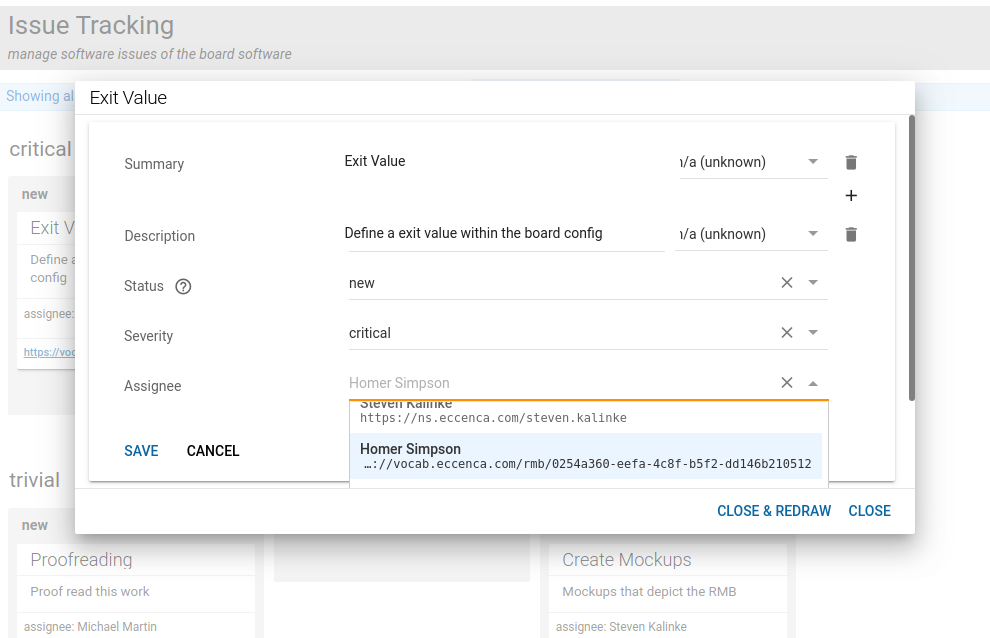
\includegraphics[width=0.90\textwidth]{img/07-SHACLINE.png}
	\caption[\tns{SHACLINE} Modal Window]{Implementation of the \tns{SHACLINE} modal window. The card \textit{Exit Value} got clicked and its Assignee value gets modified.}
	\label{fig:07SHACLINE}
\end{figure}